\documentclass[12pt]{article}
\usepackage[english]{babel}
\usepackage[utf8x]{inputenc}
\usepackage{fullpage}
\usepackage{graphicx}
\usepackage[version=3]{mhchem} 
\usepackage{siunitx} 
\usepackage{graphicx}
\usepackage{natbib} 
\usepackage{amsmath} 


\usepackage{listings}
\usepackage{color}

\title{Algorithm analyze  \\ from the time execution point of view. \\ Laboratory work nr. 1} % Title

\author{\textsc{Bîrcu} \textsc{Maxim}} % Author name

\date{\today} % Date for the report

\definecolor{mygreen}{rgb}{0,0.6,0}
\definecolor{mygray}{rgb}{0.5,0.5,0.5}
\definecolor{mymauve}{rgb}{0.58,0,0.82}

\lstset{ %
  backgroundcolor=\color{white},   % choose the background color
  basicstyle=\footnotesize,        % size of fonts used for the code
  breaklines=true,                 % automatic line breaking only at whitespace
  captionpos=b,                    % sets the caption-position to bottom
  commentstyle=\color{mygreen},    % comment style
  escapeinside={\%*}{*)},          % if you want to add LaTeX within your code
  keywordstyle=\color{blue},       % keyword style
  stringstyle=\color{mymauve},     % string literal style
}

\begin{document}


\maketitle % Insert the title, author and date

\begin{center}
\begin{tabular}{l r}

Student: & Bîrcu Maxim \\ % Partner names
Instructor: & Cojanu Irina % Instructor/supervisor

\end{tabular}
\end{center}


\section{Source code in python language.}

\lstinputlisting[language=Python]{main.py}

\section{Execution time graphs for fibonacci algorithms.}

\begin{figure}[h!]
  \centering
    {%
      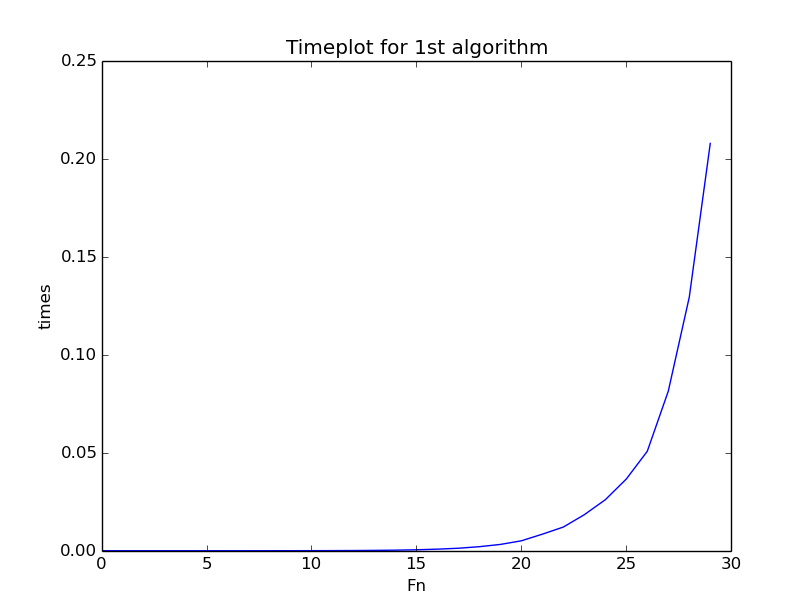
\includegraphics[width=0.5\textwidth]{figure_1}}
  \caption{Graph for first algorithm fib1()}
\end{figure}

\begin{figure}[h!]
  \centering
    {%
      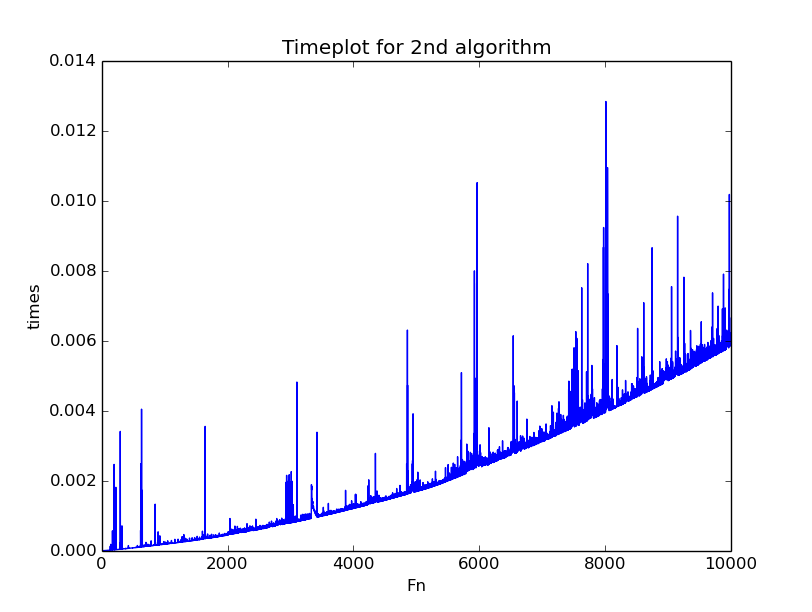
\includegraphics[width=0.5\textwidth]{figure_2}}
  \caption{Graph for second algorithm fib2()}
\end{figure}

\begin{figure}[h!]
  \centering
    {%
      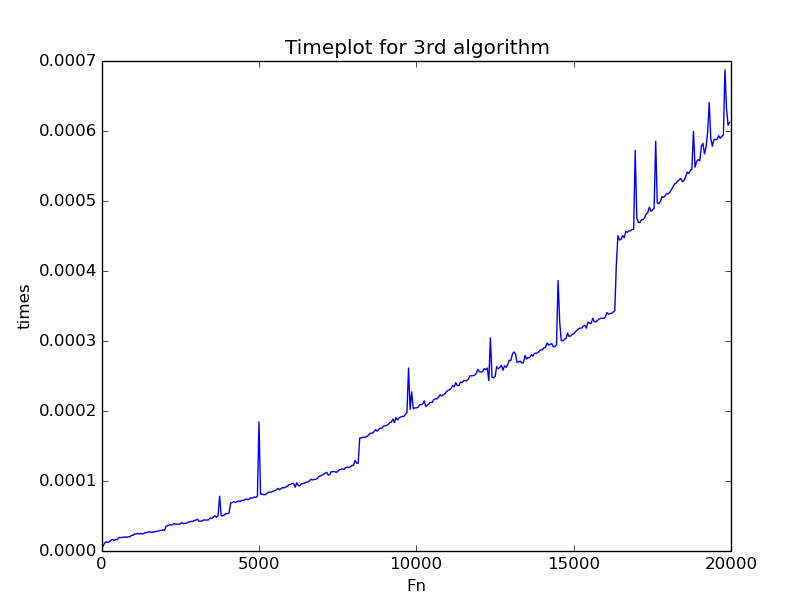
\includegraphics[width=0.5\textwidth]{figure_3}}
  \caption{Graph for third algorithm fib3()}
\end{figure}

\section{Algorithm analyze from the time execution point of view.}
\subsection{Complexity analysis for fib1 function}
We have a recursive function which number of operations is double and therefore:

\begin{center}\ce{O(Fib1(n)) = O(2^n)}\end{center}

\subsection{Complexity analysis for fib2 function}
I observed that for  for large enough input sizes the running time increases linearly, therefore we have an linearithmic function which complexity is: 
\begin{center}\ce{O(Fib2(n)) = O(n)}\end{center}

\subsection{Complexity analysis for fib3 function}

Because the number of operations is divided to 2 every frame the complexity of the algorithm is: 

\begin{center}\ce{O(Fib3(n)) = O(log2n)}\end{center}


\section{Conclusion: Sometimes we can solve a problem using a different methods and different algorithms , in this laboratory work for finding fibonacci sequence I've used 3 types of algorithms one recursive and 2 iterative and find out that recursion is an elegance method to solve the problem but from the execution time point of view , an iterative one is better  }
\end{document}